\part{Contextualização}

    \chapter{Terapia Comunitária Integrativa: Origens, Adaptações e Impactos}
        Em 1986, no bairro Pirambu, em Fortaleza, CE, a Terapia Comunitária Integrativa (TCI) teve início no Centro dos Direitos Humanos do Pirambu. Essa prática terapêutica inovadora surgiu a partir de uma rede comunitária informal. Esse movimento nasceu da união de moradores, conectados por experiências compartilhadas, resultando na criação de uma prática terapêutica significativa. 
        
        O fundador, Adalberto de Paula Barreto, doutor em psiquiatria, teologia e antropologia, desenvolveu a TCI com uma base interdisciplinar sólida, ancorada nos pilares do pensamento sistêmico, pragmática da comunicação humana, antropologia cultural, pedagogia de Paulo Freire e resiliência. Como resposta a duas necessidades essências do local: atender um grupo grande de pessoas com problemas emocionais e psíquicos semelhantes e adequar as propostas acadêmicas de promoção de saúde às carências reais apresentadas por aquela comunidade.\cite{BARRETO}
        
            \begin{quote}
            
            \textit{"A Terapia Comunitária se caracteriza por ser um grupo de ajuda mútua, um espaço de palavra, escuta e construção de vínculos com intuito de oferecer apoio a indivíduos e famílias que vivem em situações de estresse e sofrimento psíquico".}
            Adalberto de Paula Barreto
            \end{quote}
        
        Em sua essência, a metodologia da TCI  é uma jornada estruturada em fases como acolhimento, seleção da inquietação, contextualização, diálogo e partilha de experiências, enriquecimento cultural e conclusão positiva. Essa estrutura cria um espaço seguro para a expressão e ressignificação das vivências individuais e coletivas, evidenciando a transformação de carências em competências e a promoção da resiliência comunitária.\cite{SILVA}
        
        A TCI, além de promover a saúde mental, manifesta-se como um catalisador para a construção de uma sociedade consciente, solidária e participativa. Sua abordagem inclusiva valoriza a diversidade cultural e as capacidades individuais, destacando-se como força motora na formação de sujeitos sociais ativos e conscientes de seu potencial transformador.\cite{BARRETO}
        
        Além disso, a TCI responde à necessidade de uma abordagem psicossocial adaptável a diferentes contextos regionais. Em cada cenário, a TCI se adapta, considerando a capacidade humana de reagir a situações por meio de alterações na abordagem pessoal, modificação do ambiente ou uma combinação de ambas, em diferentes proporções.\cite{DANTAS} O papel de Adalberto na expansão da TCI, desde apresentações em congressos até parcerias globais, propiciaram a colaboração com setores governamentais, não governamentais e privados.\cite{GOMES}
        
        Praticada em mais de 24 países nas Américas, Europa e Ásia, a TCI é reconhecida pelo Ministério da Saúde como uma abordagem de saúde comunitária. Integrada à Política Nacional de Práticas Integrativas e Complementares (PNPIC) desde 2017, a TCI combina conhecimento científico e sabedoria popular na busca de soluções para conflitos e sofrimentos humanos.\cite{ABRATECOM}
        
        A Associação Brasileira de Terapia Comunitária Integrativa (ABRATECOM), autorizada por seu criador desde 2004, executa um papel fundamental nesse cenário. Atualmente, computa mais de 30.500 terapeutas comunitários credenciados, em todo o Brasil, destacando a amplitude e o alcance dessa prática.\cite{SILVAFRANCO} Abaixo a distribuição geográfica dos Polos Formadores e de Cuidado credenciados pela\cite{ABRATECOM}:
        
            \begin{figure}[!h] % ambiente usado para inserção de imagens
                \centering
                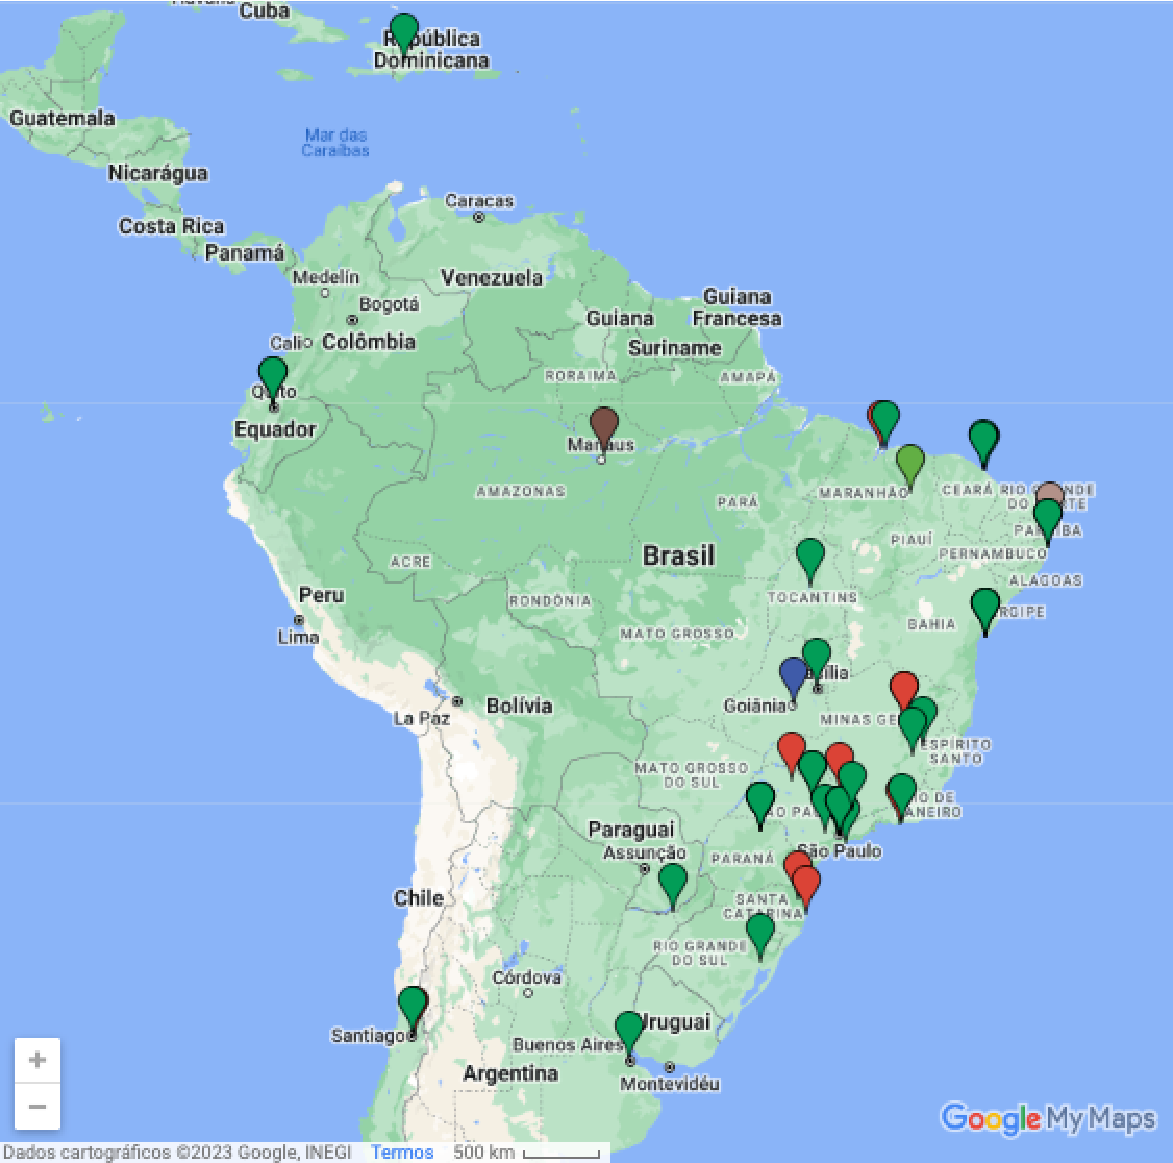
\includegraphics[scale=0.7]{latex/figuras/polos.pdf}
                \caption[Distribuição de Polos Formadores ABRATECOM]%seção
                {Distribuição de Polos Formadores e de Cuidado}%legenda
            \end{figure}
        
        Em 2020, frente aos desafios da pandemia da COVID-19, a TCI abraçou a era digital. No Polo Formador Afinando Vidas, rodas experimentais online foram conduzidas para criar e validar um protocolo adaptado das etapas da TCI. Essa adaptação não apenas ressignificou a concepção de contato social e cuidado, mas também promoveu uma nova e mais ampla forma de conexão, mantendo os valores fundamentais da prática. \cite{SILVAeOTAVIANO}
        
        Os valores que sustentam a TCI - acolhimento, simplicidade, circularidade do cuidado, valorização das emoções, ousadia e transgressão, geração de dúvidas nas convicções, horizontalidade das relações, percepção do outro como recurso, aceitação da imprevisibilidade e amor com bom humor - são pilares que moldam e fortalecem essa prática transformadora.\cite{SILVA}
        
        \cite{BOARETTO} em um estudo quase-experimental, realizado entre agosto de 2018 e abril de 2019, avaliaram os níveis de possível ansiedade e depressão, em estudantes de uma universidade pública, durante sessões de TCI. Participaram 25 estudantes, divididos em quatro grupos, com coleta de dados antes e depois das sessões. Inicialmente, os escores para possível ansiedade eram de 52\%, e para depressão, de 12\%.
        
            \begin{figure}[!h] % ambiente usado para inserção de imagens
                \centering
                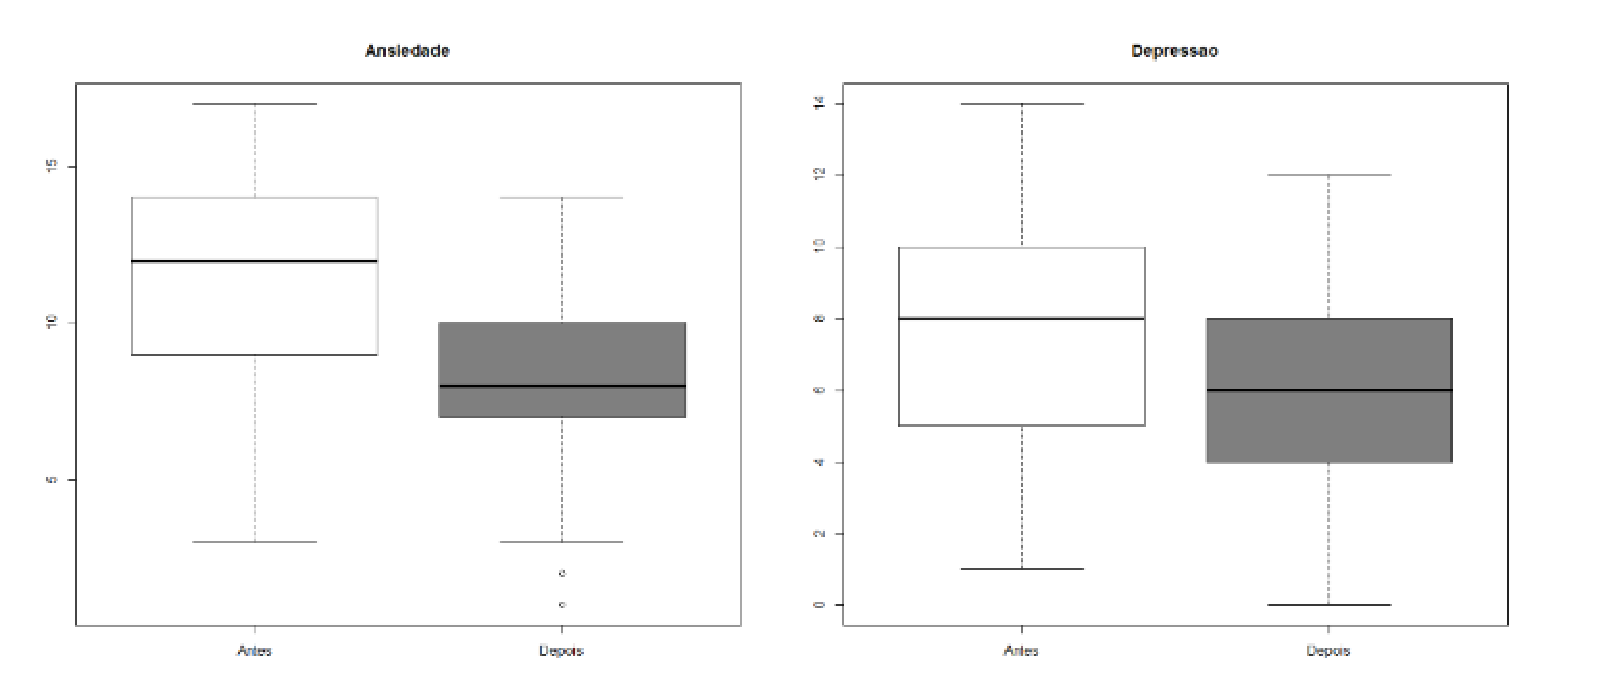
\includegraphics[scale=0.5]{latex/figuras/boaretto.pdf}
                \caption[Níveis de Ansiedade e Depressão]%seção
                {Comparação dos níveis do escore antes e depois para possível ansiedade e depressão. \cite{BOARETTO}}%legenda
            \end{figure}
        
        Ao analisar os dados, comparando o antes e depois de cinco rodas de TCI, os resultados foram notáveis, destacando a eficácia da TCI na redução desses índices, evidenciando sua relevância e impacto positivo na saúde mental, isso evidencia a necessidade e importância de programas de intervenção psicoterápicas dentro das universidades.\cite{BOARETTO}
        
        Em outra aplicação prática, indicadora dos benefícios da TCI, foi observada em uma pesquisa realizada para avaliar os efeitos antes e depois de uma única sessão. Um caso envolveu uma senhora que frequentava as rodas de forma assídua e enfrentava, em casa, de forma recorrente, a difícil situação de ter uma sobrinha envolvida com drogas, sendo essa sua única família. A sobrinha encorajada a participar da roda de TCI, permaneceu em silêncio durante toda a sessão, mas ao final, expressou que "a terapia não é um lugar de covardes". Sua avaliação antes da sessão refletia um estado emocional fragilizado, enquanto após a TCI, ela se sentia com disposição para explorar novas perspectivas e caminhos.\cite{LEITEePALOS}Isso ilustra a TCI não apenas como um espaço de expressão, mas também como um facilitador de perspectivas de mudança e crescimento em situações complexas.
        
        Em resumo, a Terapia Comunitária Integrativa não é apenas uma prática terapêutica, é uma força catalisadora que transcende fronteiras, promovendo saúde mental, fortalecendo comunidades e gerando transformações positivas. Seja nas rodas presenciais ou adaptadas para o ambiente digital, a TCI continua a ser uma fonte poderosa de conexão, cura e crescimento, iluminando caminhos para um mundo mais resiliente e compassivo.
    
    \chapter{Engenharia Eletrônica na Saúde Mental: Inovações Tecnológicas e Transformação de Práticas Terapêuticas}
        A constante preocupação com a saúde da população e os avanços tecnológicos permitiram o desenvolvimento e integração de recursos que aprimoram a eficiência do cuidado. Destaca-se a atuação e os avanços proporcionados pela engenharia eletrônica no cuidado com a saúde mental, moldando uma abordagem de intervenção que se estende para a vida diária do indivíduo. Essa expansão visa potencializar a eficácia dos tratamentos terapêuticos.
        
        A engenharia eletrônica desempenha um papel essencial no comprometimento com a expansão e manutenção da saúde mental. O desenvolvimento de tecnologias inovadoras oferece uma contribuição significativa por meio de sensores, algoritmos de processamento de sinais, softwares avançados, equipamentos eletrônicos e dispositivos vestíveis (\textit{Wearables}). Essas ferramentas proporcionam intervenções personalizadas e direcionadas, facilitando a atuação de profissionais da saúde mental com abordagens mais precisas.
        
        As abordagens se estendem de maneiras ativas, transformando a percepção do tratamento de distúrbios mentais. Ao integrar a tecnologia como complemento, estudos de caso e exemplos práticos destacam um potencial revolucionário na transformação do panorama geral da saúde mental.
        
        Os recentes avanços em Inteligência Artificial (IA) e Processamento de Linguagem Natural (PNL) transformaram a análise de notas clínicas e \textit{insights} do Registro Eletrônico de Saúde(EHR). Um estudo britânico aplicou PNL e IA no tratamento da depressão, identificando padrões de comportamento que demandam intervenção. Ao prever crises em pacientes de saúde mental, a pesquisa revelou a viabilidade técnica dessas abordagens, destacando oportunidades de integração em ferramentas de apoio à decisão clínica local\cite{MSOSA}.
        
        No campo da neuroestimulação elétrica, estudos oferecem uma abordagem inovadora para tratar distúrbios mentais, modulando diretamente a sincronia oscilatória e a conectividade entre regiões cerebrais específicas. Essa técnica promissora representa um avanço significativo no tratamento, atuando no nível cerebral para alterar circuitos envolvidos em distúrbios neuropsiquiátricos\cite{LO}.
        
        Outro exemplo prático envolve a proposta de um Assistente de Monitoramento de Emoções e Mentalidade (EMMA), um \textit{chatbot} eficiente para saúde mental. Utilizando \textit{Deep Learning} para analisar emoções por meio de texto, voz e expressão facial, alcançou impressionantes 85\% de precisão. A implementação de tecnologia \textit{blockchain} assegura a segurança dos registros eletrônicos, permitindo o compartilhamento seguro com profissionais de saúde. Essa abordagem visa uma gestão eficaz de problemas de saúde mental de forma mais presente e com menor demanda de recursos\cite{EMMA}.
        
        Esses exemplos reforçam a importância da engenharia eletrônica no desenvolvimento de práticas de cuidado com a saúde mental, por meio de inovações tecnológicas, proporcionando soluções eficazes e personalizadas para o bem-estar emocional. Na área de abordagem em saúde comunitária, destaca-se a Terapia Comunitária Integrativa, recentemente adaptada para a forma online\cite{SILVAFRANCO}. A engenharia eletrônica desempenha um papel crucial no desenvolvimento de uma plataforma online, segura e eficiente, capaz de facilitar os encontros terapêuticos comunitários de forma remota. Isso inclui a possibilidade de gerenciar sessões e integrar tecnologias de comunicação, como sistemas de videoconferência, proporcionando uma experiência fluida para terapeutas comunitários e participantes.
        
        A preocupação com a segurança da informação é primordial para engenheiros eletrônicos. Por isso, na construção de uma plataforma online, incorpora-se um compromisso rigoroso com a transparência no tratamento de dados sensíveis dos usuários. Esse compromisso abrange o respeito à privacidade, a consideração cuidadosa da necessidade e segurança dos dados coletados, e a intenção contínua de estar em conformidade com a Lei Geral de Proteção de Dados\cite{LGPD}. Essa abordagem reforça a confiança dos usuários na plataforma, assegurando que suas informações sejam tratadas com o mais alto padrão de tecnologias de segurança e em conformidade com as leis vigentes.
        
        Adicionalmente, para a engenharia eletrônica, é essencial implementar uma análise de dados de usabilidade para a identificação e resolução de problemas, além de orientar as tomadas de decisões informadas. Essas decisões têm como objetivo identificar, otimizar, melhorar e manter o desempenho dos sistemas, impulsionando a inovação contínua. Essa abordagem é fundamental para assegurar que a plataforma seja intuitiva e facilite a interação dos usuários, atendendo, assim, às necessidades específicas requeridas pela TCI online.
        
        Por meio de suas inovações, a engenharia eletrônica desempenha um papel vital na criação de intervenções personalizadas voltadas para o bem-estar emocional. Essa sinergia entre tecnologia e a dedicação ao cuidado mental possibilita a elaboração de uma plataforma destinada ao gerenciamento das sessões online de Terapia Comunitária Integrativa. Nessa abordagem, a engenharia eletrônica não apenas estabelece uma base robusta, mas também facilita e aprimora a experiência de cada participante de maneira significativa.
        
    \chapter{Conectando Comunidades: A Integração da Terapia Comunitária Integrativa na Plataforma Online}
    
        A integração da Terapia Comunitária Integrativa Online na plataforma ocorre por meio da incorporação de algumas características também utilizadas na psicoterapia online e na psicoterapia baseada na internet. Essa abordagem inovadora tem proporcionado benefícios significativos, tornando as rodas de TCI mais acessíveis a um público mais amplo e diversificado, superando barreiras geográficas e adaptando-se à disponibilidade dos participantes.
        
        Na terapia online, as pessoas podem participar de sessões terapêuticas remotamente, de forma síncrona, independentemente de sua localização física. Essa prática foi implementada na TCI online não apenas para facilitar a participação de pessoas com diferentes origens, culturas e rotinas, mas também para oferecer flexibilidade de horários tanto para terapeutas quanto para participantes. Além disso, a plataforma favorece a criação de salas de videoconferência no \textit{Google Meet}, que possui recursos tecnológicos que aproximam os participantes, auxiliando na criação de laços, gerando identificação e apoio mútuo que podem se estender para além das sessões online.
        
        A psicoterapia baseada na internet foi integrada à plataforma por meio de uma página com vídeos acessíveis a qualquer momento. Esse recurso visa enriquecer culturalmente e promover uma sensação de bem-estar sempre que o usuário desejar, contribuindo para a consciência pessoal durante momentos de tranquilidade e a manutenção de práticas que também são exercidas nas rodas de TCI online.
        
        A proposta de criar links automatizados do \textit{Google Meet} para as Rodas de TCI remotas facilita o gerenciamento das sessões pelos terapeutas. Ao pré-determinar datas e horários, sincronizando automaticamente com o Google Calendar, os terapeutas comunitários otimizam seu tempo, permitindo dedicação a atividades enriquecedoras. Para os participantes, a proposta oferece uma organização clara dos horários e datas das rodas de TCI online, proporcionando autonomia na escolha das sessões terapêuticas que mais se adequam às suas rotinas.
        
        A abordagem da Terapia Comunitária Integrativa promove um enfoque intercultural, celebrando a diversidade e incentivando o envolvimento ativo dos membros da comunidade. Reconhecendo a relação intrínseca entre desenvolvimento humano e contextos culturais, a TCI conta com o papel adaptativo do terapeuta comunitário para manter o diálogo aberto e respeitoso, garantindo que a qualidade das interações em um grupo remoto seja equivalente a um grupo presencial.
        
        Nas sessões online, a plataforma oferece uma experiência aprimorada, permitindo reunir pessoas para as rodas de psicoterapia comunitária integrativa por meio da tecnologia. O redirecionamento para a plataforma do \textit{Google Meet} facilita a interação, criando um espaço virtual acolhedor onde os participantes podem compartilhar suas histórias e momentos, sem julgamentos.
        
        A possibilidade de compartilhar recursos multimídia, por meio de uma \textit{playlist} de vídeos no \textit{YouTube} conectada à plataforma, enriquece a experiência terapêutica. Essa tecnologia apoia visualmente o processo terapêutico, proporcionando bem-estar e valorização cultural em momentos além das sessões de terapia.
        
        Esses elementos, entrelaçados por representações que geram identificações, formam a base para um processo de cura significativo, potencializando mudanças individuais e comunitárias. A plataforma de TCI online promove a compreensão e integração ativa das diversas dimensões culturais, valorizando a diversidade como essencial para o bem-estar emocional e social da comunidade.
        
        Os avanços na tecnologia e na comunicação têm permitido a inclusão de recursos que favorecem a manutenção da saúde mental. É fundamental destacar que a concepção de saúde é profundamente influenciada pela cultura, e a TCI reconhece e respeita essas diversas visões de mundo. Além disso, a Terapia Comunitária Integrativa defende a sintonia do indivíduo com as emoções e sentimentos despertados pelo contato, exigindo uma elevada auto-percepção. Incentiva a disposição para ouvir e compreender o outro, abrindo espaço para novas perspectivas e ressignificações daquilo que anteriormente era considerado imutável ou insuperável. Isso promove um ambiente propício ao crescimento pessoal e à construção de relações mais saudáveis, consolidando a visão integral da plataforma como um facilitador de bem-estar emocional e social.
    
    %\chapter{Engenharia Eletrônica na Implementação da Plataforma}
    % \section{Exploração das contribuições específicas da Engenharia Eletrônica no desenvolvimento da plataforma.}
    % \section{Destaque de tecnologias e recursos eletrônicos que podem ser aplicados.}
    
    \chapter{Considerações Éticas e Privacidade de Dados no Cuidado da Saúde Mental Online}
    
        Nos últimos anos, as inovações tecnológicas têm desempenhado um papel crucial na evolução dos serviços de atenção a saúde mental, essa crescente demanda aliada às possibilidades oferecidas pela tecnologia, resultou no desenvolvimento de novas modalidades de atendimento psicológico. O Conselho Federal de Psicologia (CFP), reconhecendo a importância desse avanço, regulamentou o atendimento psicoterápico remoto como uma prática profissional permitida e readequou a resolução em 2020 para atender o contexto mundial frente à crise sanitária provocada pela Covid-19\cite{CFP}.
        
        Os atendimentos psicológicos online têm se destacado pela eficácia técnica, ampliando o alcance dos serviços de atenção à saúde mental. Essa modalidade adapta o cuidado sem necessidade de contato presencial, garantindo resultados efetivos, como a melhoria do bem-estar emocional, e observando os aspectos éticos e legais inerentes ao cuidado mental\cite{SIEGMUND}.
        
        A Terapia Comunitária Integrativa (TCI), reconhecida pelo Ministério da Saúde como uma abordagem psicossocial avançada, também abraçou a era digital. O Polo Formador em TCI Afinando Vidas, diante dos desafios impostos pela pandemia, promoveu rodas experimentais online, resultando na criação de um protocolo de mediação das rodas. Esse protocolo foi replicado nacionalmente pela ABRATECOM, permitindo ressignificar a concepção de presença e cuidado, promovendo uma nova forma de conexão comunitária\cite{SILVAeOTAVIANO}.
        
        A convergência entre o cuidado mental e a tecnologia na plataforma desenvolvida destaca a sinergia entre essas áreas. A interdisciplinaridade contribui significativamente para o aprimoramento mútuo, garantindo práticas éticas na Terapia Comunitária Integrativa online. Essa transição para o ambiente virtual exigiu uma reinvenção na abordagem terapêutica, visando continuar a promoção da formação de laços sociais solidários, conexões e qualidade de vida, agora sem a necessidade de contato presencial. A estrutura da plataforma, construída com base nas APIs do Google, não apenas garante a segurança, mas também preserva a privacidade dos usuários, permitindo que explorem os benefícios da TCI online com tranquilidade.
        
        A segurança dos dados torna-se uma prioridade na oferta de serviços psicológicos online, alinhando-se com a Lei Geral de Proteção de Dados (LGPD), legislação brasileira que regulamenta o tratamento de dados pessoais. Os principais princípios da \cite{LGPD} foram incorporados na construção da plataforma, incluindo a transparência no tratamento dos dados, o respeito à privacidade, a finalidade específica do uso dos dados, a necessidade e a segurança dos dados coletados. Essa medida foi adotada para garantir a conformidade com as normas de proteção de dados e para que a dinâmica dos grupos de TCI online continue a promover a diversidade, cultura, escuta ativa e respeito mútuo.
        
        Ao consultar as políticas do \textit{OAuth} 2.0 do Google, foram adotadas medidas rigorosas para atender aos requisitos mínimos de segurança e privacidade. Durante a autenticação, apenas os escopos necessários foram solicitados, minimizando o acesso aos dados do usuário. A revogação manual do acesso é permitida pela plataforma, demonstrando mais um compromisso com a privacidade dos usuários\cite{OAUTHSCOPES}.
        
        Em resumo, a plataforma não apenas integra efetivamente a Terapia Comunitária Integrativa (TCI) à tecnologia, mas também responde de maneira ética e centrada na comunidade, às demandas contemporâneas de saúde mental. A seleção cuidadosa das tecnologias implementadas não só garante confidencialidade, privacidade e ética, mas também molda uma experiência que contribui significativamente para o bem-estar e desenvolvimento pessoal dos usuários. Essa abordagem destaca a plataforma como um avanço notável no campo de gerenciamento das rodas de Terapia Comunitária Integrativa online, oferecendo uma resposta inovadora e cuidadosa às necessidades da saúde mental moderna.